\section{Prediction Performance of HDP}
\label{sec:Result}
In this section, we present the experimental results of the HDP approach to address RQ1.

{\bf RQ1: Is heterogeneous defect prediction comparable to WPDP and existing CPDP approaches for heterogeneous metric sets (CPDP-CM and CPDP-IFS)?}

RQ1 leads us to investigate whether our
HDP is comparable to WPDP (Baseline1), CPDP-CM
(Baseline2), and CDDP-IFS (Baseline3)~\cite{He14}. We report the representative HDP results in Section~\ref{subsec01},~\ref{subsec02}, and~\ref{subsec03} based on Gain ratio attribute selection for metric selection, KSAnalyzer with the cutoff threshold of 0.05, and Simple logistic classifier. Among different
metric selections, Gain ratio attribute selection with Simple logistic led to the best
prediction performance overall. In terms of analyzers, KSAnalyzer led to the best prediction performance.
Since the KSAnalyzer is based on the p-value of a statistical test, we chose a cutoff of 0.05 which is a commonly accepted significance level in the
statistical test~\cite{Corder09}.

In Section~\ref{subsec04},~\ref{subsec05}, and~\ref{subsec06}, we report the HDP results by using various metric selection approaches, metric matching analyzers, and machine learners respectively to investigate HDP performances more in terms of RQ1.

%----------------------------------------------------------
\subsection{Comparison Result with Baselines}
\label{subsec01}% KSAnalyzer with the cutoff of %
% 0.05}
%----------------------------------------------------------

\begin{table}[!t]
%\footnotesize
%\small
%\scriptsize
\centering
\caption{Comparison results among WPDP, CPDP-CM, CPDP-IFS,
and HDP by KSAnalyzer with the cutoff of 0.05 in a median AUC. (Cliff's $\delta$ magnitude --- N: Negligible, S: Small, M: Medium, and L: Large)
%  Outperforming results with statistical
%  significance (Wilcoxon signed-rank test, p$<$0.05) between within and cross by
%  the proposed approach and between cross using common features and those by the
%  proposed approach are bold-faced and underlined respectively.
}
\label{tab:result_overview}
%\setlength{\tabcolsep}{5pt}
%\setlength{\extrarowheight}{1.5pt}
%\begin{tabular}{|@{ }c@{ }||@{}c@{}|@{}c@{}|@{}c@{}||@{}c@{}|}
\begin{tabular}{|@{}c@{}||@{}C{21mm}@{}|@{}C{21mm}@{}|@{}C{21mm}@{}||@{}C{8mm}@{}|}
\hline
{\bf Target}
& \specialcell{{\bf WPDP}\\{(Baseline1)}} 
&\specialcell{{\bf CPDP-CM}\\{(Baseline2)}}
&\specialcell{{\bf CPDP-IFS}\\{(Baseline3)}}
&\specialcell{{\bf HDP}\\{\bf KS}}%\\{cutoff=0.05}}
\\
\hline \hline
EQ	&0.583 (0.997,{\bf L})	&0.776 (0.178,{\bf S})	&0.461 (1.000,{\bf L})	&{\bf 0.782}* \\ \hline
JDT	&{\bf 0.795} (-0.533,L)	&0.781 (0.164,{\bf S})	&0.543 (0.999,{\bf L})	&0.767* \\ \hline
LC	&0.575 (0.397,{\bf M})	&0.636 (0.059,{\bf N})	&0.584 (0.198,{\bf S})	&0.655 \\ \hline
ML	&{\bf 0.734} (-0.762,L)	&0.651 (0.642,{\bf L})	&0.557 (0.999,{\bf L})	&0.692* \\ \hline
PDE	&0.684 (0.279,{\bf S})	&0.681 (0.211,{\bf S})	&0.566 (0.966,{\bf L})	&0.693* \\ \hline
Apache	&0.715 (0.044,{\bf N})	&0.697 (0.255,{\bf S})	&0.618 (0.582,{\bf L})	&0.731* \\ \hline
Safe	&0.706 (0.583,{\bf L})	&0.749 (0.388,{\bf M})	&0.630 (0.698,{\bf L})	&\underline{{\bf 0.837}}* \\ \hline
Zxing	&0.605 (0.678,{\bf L})	&0.618 (0.529,{\bf L})	&0.556 (0.652,{\bf L})	&{\bf 0.650}* \\ \hline
ant-1.3	&0.609 (0.707,{\bf L})	&0.781 (0.222,{\bf S})	&0.528 (0.713,{\bf L})	&{\bf 0.800}* \\ \hline
arc	&0.670 (0.213,{\bf S})	&0.626 (0.524,{\bf L})	&0.547 (0.954,{\bf L})	&0.701 \\ \hline
camel-1.0	&0.550 (0.427,{\bf M})	&0.590 (0.397,{\bf M})	&0.500 (0.600,{\bf L})	&0.639* \\ \hline
poi-1.5	&0.707 (-0.010,{\bf N})	&0.675 (0.298,{\bf S})	&0.640 (0.571,{\bf L})	&0.723 \\ \hline
redaktor	&{\bf 0.745} (-0.900,L)	&0.496 (0.085,{\bf N})	&0.489 (0.274,{\bf S})	&0.528 \\ \hline
skarbonka	&0.569 (0.524,{\bf L})	&0.744 (-0.152,S)	&0.540 (0.536,{\bf L})	&{\bf 0.689}* \\ \hline
tomcat	&{\bf 0.778} (-0.614,L)	&0.675 (0.962,{\bf L})	&0.608 (1.000,{\bf L})	&\underline{0.737}* \\ \hline
velocity-1.4	&{\bf 0.725} (-0.984,L)	&0.412 (-0.142,{\bf N})	&0.429 (-0.138,{\bf N})	&0.391 \\ \hline
xalan-2.4	&{\bf 0.755} (-0.932,L)	&0.658 (0.405,{\bf M})	&0.499 (0.999,{\bf L})	&\underline{0.673}* \\ \hline
xerces-1.2	&0.624 (-0.954,L)	&0.462 (0.304,{\bf S})	&0.473 (0.115,{\bf N})	&0.486 \\ \hline
cm1	&0.653 (0.344,{\bf M})	&0.597 (0.520,{\bf L})	&0.554 (0.737,{\bf L})	&0.720* \\ \hline
mw1	&0.612 (0.515,{\bf L})	&0.518 (0.488,{\bf L})	&0.621 (0.401,{\bf M})	&0.745 \\ \hline
pc1	&{\bf 0.788} (-0.323,S)	&0.666 (0.812,{\bf L})	&0.557 (0.997,{\bf L})	&\underline{0.751}* \\ \hline
pc3	&{\bf 0.794} (-0.830,L)	&0.665 (0.810,{\bf L})	&0.511 (1.000,{\bf L})	&\underline{0.738}* \\ \hline
pc4	&{\bf 0.900} (-1.000,L)	&0.624 (0.221,{\bf S})	&0.590 (0.955,{\bf L})	&0.681* \\ \hline
jm1	&{\bf 0.705} (-0.680,L)	&0.571 (0.688,{\bf L})	&0.563 (0.997,{\bf L})	&\underline{0.688}* \\ \hline
pc2	&0.748 (0.819,{\bf L})	&0.634 (0.805,{\bf L})	&0.474 (0.992,{\bf L})	&\underline{{\bf 0.893}}* \\ \hline
pc5	&{\bf 0.954} (-0.364,M)	&0.841 (0.999,{\bf L})	&0.260 (0.999,{\bf L})	&\underline{0.950}* \\ \hline
mc1	&0.863 (0.504,{\bf L})	&0.832 (0.970,{\bf L})	&0.224 (0.999,{\bf L})	&\underline{{\bf 0.893}}* \\ \hline
mc2	&0.646 (0.292,{\bf S})	&0.536 (0.772,{\bf L})	&0.515 (0.699,{\bf L})	&\underline{{\bf 0.686}}* \\ \hline
kc3	&0.609 (0.382,{\bf M})	&0.636 (0.313,{\bf S})	&0.568 (0.680,{\bf L})	&\underline{{\bf 0.678}}* \\ \hline
ar1	&0.582 (0.680,{\bf L})	&0.464 (0.829,{\bf L})	&0.586 (0.555,{\bf L})	&\underline{{\bf 0.736}}* \\ \hline
ar3	&0.574 (0.860,{\bf L})	&0.839 (0.295,{\bf S})	&0.664 (0.572,{\bf L})	&{\bf 0.835}* \\ \hline
ar4	&0.657 (0.880,{\bf L})	&0.588 (0.801,{\bf L})	&0.570 (0.819,{\bf L})	&\underline{{\bf 0.812}}* \\ \hline
ar5	&0.804 (0.576,{\bf L})	&0.875 (0.474,{\bf L})	&0.766 (0.550,{\bf L})	&\underline{{\bf 0.911}}* \\ \hline
ar6	&0.654 (0.072,{\bf N})	&0.613 (0.378,{\bf M})	&0.524 (0.497,{\bf L})	&\underline{0.667}* \\ \hline
\hline
{\bf {\em All}}	&0.654		&0.632		&0.558		&\underline{{\bf 0.718}}*
\\ \hline
%{\bf {\em All}} & 0.657 & 0.636 &0.555	& \underline{\bf 0.724}*  \\ \hline \hline

%{\bf {\em Cliff's $\delta$}} & \specialcell{0.143\\(Negligible)} & \specialcell{0.296\\(Small)} & \specialcell{0.792\\(Large)}	& --  \\ \hline


\end{tabular}
\end{table}

% 
% \begin{figure*}[t]
% 	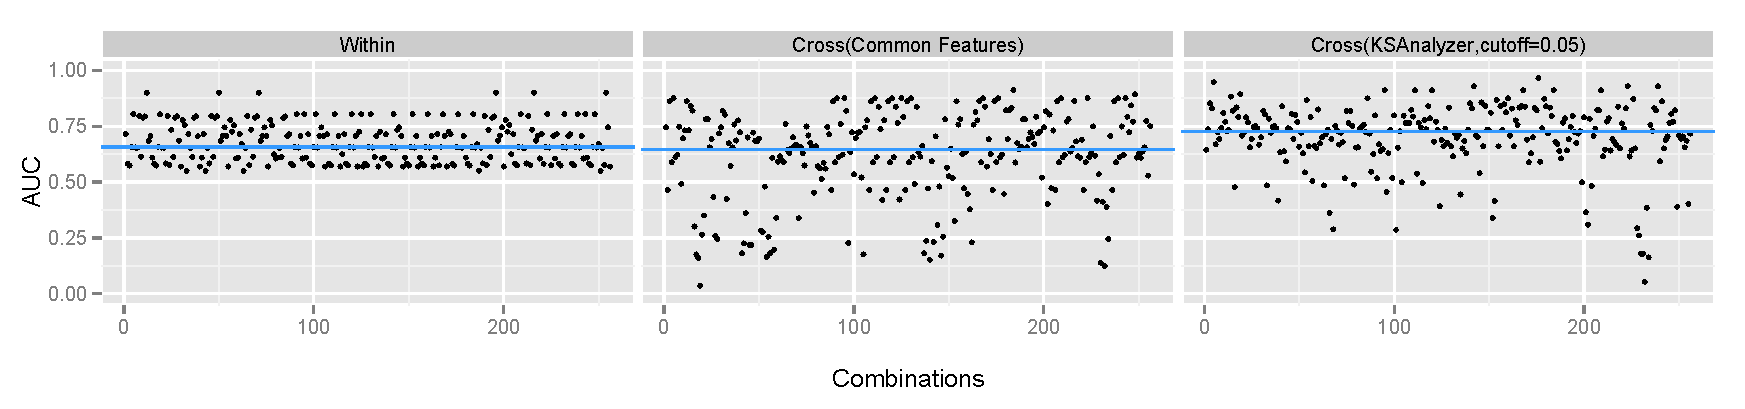
\includegraphics[width=\linewidth]{Figures/Result/auc_compare.pdf}
% 	\caption{Prediction performance variance among within-prediction,
% 	cross-prediction using common metrics, and cross-prediction by KSAnalyzer with
% 	the cutoff of 0.05 in terms of AUC. The number of prediction combinations is 256.}
% 	\label{fig:compare_results_on_defect}
% \end{figure*}


Table~\ref{tab:result_overview} shows the prediction performance (a median AUC)
of baselines and HDP by KSAnalyzer with the cutoff of 0.05 and Cliff's $\delta$ with its magnitude
for each target. The last row, {\em all} targets, show an overall prediction performance of baslines and HDP in a median AUC. Baseline1 represents
the WPDP results of a target project and Baseline2 shows
the CPDP results using common metrics (CPDP-CM) between source and target
projects. Baseline3 shows the results of CPDP-IFS proposed by He et
al.~\cite{He14}. The last column shows the HDP results by KSAnalyzer with the
cutoff of 0.05. If there are better results between Baseline1 and our approach with statistical significance (Wilcoxon signed-rank
test~\cite{Wilcoxon45}, p$<$0.05), the better AUC values are in
bold font as shown in Table~\ref{tab:result_overview}.
Between Baseline2 and our approach, better AUC values with
statistical significance are underlined in
the table. Between Baseline3 and our approach, better AUC values with
statistical significance are shown with an asterisk (*).

The values in parentheses in Table~\ref{tab:result_overview} show Cliff's $\delta$ and its magnitude for the effect size among baselines and HDP. If a Cliff's $\delta$ is a positive value, HDP improves a baseline in terms of the effect size. As explained in Section~\ref{sec:measure}, based on a Cliff's $\delta$, we can estimate the magnitude of the effect size (N: Negligible, S: Small, M: Medium, and L: Large). For example, the Cliff's $\delta$ of AUCs between WPDP and HDP for EQ is 0.997 and its magnitude is {\em Large} as in Table~\ref{tab:result_overview}. In other words, HDP outperforms WPDP in EQ in terms of the effect size.

%From Table~\ref{tab:result_overview}, 
We observed the following results about RQ1:
\squishlist
	\item In 23 out of 34 targets, HDP by KSAnalyzer with the cutoff of
	0.05 leads to better or comparable results against WPDP with statistical
	significance. (The WPDP results in only JDT, ML, redaktor, tomcat, velocity-1.4, xalan, pc1, pc3, pc4, jm1, and pc5 are in bold font.)
	\item HDP by KSAnalyzer with the cutoff of 0.05 outperforms
	WPDP with statistical significance when considering
	results from all targets ({\em All} in the second last row in the table) together in
	our experimental settings.
	\item The Cliff's $\delta$ values between WPDP and HDP are positive in 21 out of 34 targets. In about 62\% of targets, HDP shows comparable or better results to HDP in terms of effect size.
	\item HDP by KSAnalyzer with the cutoff of 0.05
	leads to better or comparable results to CPDP-CM
	with statistical significance. (no underlines in CPDP-CM of
	Table~\ref{tab:result_overview})
	\item HDP by KSAnalyzer with the cutoff of 0.05 outperforms
	CPDP-CM with statistical significance
	when considering results from {\em All} targets in our experimental
	settings.
	\item The Cliff's $\delta$ values between CPDP-CM and HDP are positive in 32 out 34 targets. In other words, HDP improves CPDP-CM in most targets in terms of effect size.
	\item HDP by KSAnalyzer with the cutoff of 0.05
	leads to better or comparable results to CPDP-IFS with
	statistical significance. (no asterisks in CPDP-IFS of
	Table~\ref{tab:result_overview})
	\item HDP by KSAnalyzer with the cutoff of 0.05 outperforms
	CPDP-IFS with statistical significance
	when considering results from {\em All} targets in our experimental
	settings.
	\item The Cliff's $\delta$ values between CPDP-IFS and HDP are positive in all targets except for velocity-1.4.
\squishend

% Figure~\ref{fig:compare_results_on_defect} shows how the prediction performance
% of within- and cross-prediction varies. In
% Figure~\ref{fig:compare_results_on_defect}, each dot represents a prediction
% combination, e.g, EQ$\Rightarrow$Apache. In total, 222 dots (prediction
% combinations) are shown in each plot of the figure. The solid line in
% the figure represents the overall prediction performance, i.e. the median AUC
% values for prediction combinations.
% 
% Cross-results using common
% metrics show unstable results with large variance as in
% Figure~\ref{fig:compare_results_on_defect} where many prediction results are
% plotted under the AUC of 0.5.
% In addition, the median AUC (0.636) in cross-results using common metrics is
% slightly worse than that (0.657) in within-results. 
% 
% In cross-prediction by KSAnalyzer, some results are also plotted under the
% AUC of 0.5 because some cross-results by KSAnalyzer in the
% projects such as velocity-1.4 and xerces-1.2 have relatively low AUCs
% as shown in Table~\ref{tab:result_overview}.
% 
% However, note that the results by KSAnalyzer
% led to the best prediction performance in the median AUC and the variance of
% the results is smaller than cross-results using common metrics in
% Figure~\ref{fig:compare_results_on_defect}. The cross-result (0.724) of
% KSAanalyzer with the cutoff of 0.05 outperforms the within-result
% (0.657) and cross-result using common metrics (0.636) with statistical
% significance.

% We also compare
% cross-prediction results of AS, random analyzer, and manual matching as well. As we observe, the cross-result of AS outperforms that of both random analyzer and manual matching.

% \begin{table*}[t]
% \small
% \centering
% \caption{Within and cross-prediction results in median AUCs on various cutoff
% values. (W.=Within, C.=Cross) Better results between within- and
% cross-predictions are bold-faced (Mann-Whitney U-test, p$<$0.05).}
% \label{tab:DiffCutOffs}
% %\setlength{\tabcolsep}{5pt}
% %\setlength{\extrarowheight}{1.5pt}
% \begin{tabular}{|@{ }c@{ }||@{ }c@{ }|@{ }c@{ }|@{ }c@{ }||@{ }c@{
% }|@{ }c@{ }|@{ }c@{ }||@{ }c@{ }|@{ }c@{ }|@{ }c@{ }||@{ }c@{ }|@{ }c@{ }|@{
% }c@{ }|}
% \hline
% \multirow{2}{*}{{\bf Cutoffs}}	& \multicolumn{3}{c||}{{\bf PAnalyzer}} &
% \multicolumn{3}{c||}{{\bf KSAnalyzer}} &
% \multicolumn{3}{c||}{{\bf SCoAnalyzer}} &
% \multicolumn{3}{c|}{{\bf PiAnalyzer}} \\\cline{2-13}
% 	& {\bf W. AUC} & {\bf C. AUC} & {\bf \# comb.}
% 	& {\bf W. AUC} & {\bf C. AUC} & {\bf \# comb.}
% 	& {\bf W. AUC} & {\bf C. AUC} & {\bf \# comb.}
% 	& {\bf W. AUC} & {\bf C. AUC} & {\bf \# comb.} \\\hline
% \hline
% 0.00 & {\bf 0.683} & 0.641 & 600 & 0.664 & 0.686 & 548 & {\bf 0.683} & 0.601 &
% 600 & {\bf 0.683} & 0.612 & 600\\ \hline 0.05 & {\bf 0.683} & 0.658 & 600 & 0.649 & {\bf 0.729} & 249 & {\bf 0.683} & 0.601 & 600 & {\bf 0.683} & 0.612 & 600\\ \hline
% 0.10 & {\bf 0.683} & 0.660 & 600 & 0.647 & {\bf 0.740} & 202 & {\bf 0.683} & 0.601 & 600 & {\bf 0.683} & 0.612 & 600\\ \hline
% 0.20 & {\bf 0.683} & 0.668 & 587 & 0.657 & {\bf 0.746} & 144 & {\bf 0.683} & 0.601 & 600 & {\bf 0.683} & 0.611 & 600\\ \hline
% 0.30 & 0.683 & 0.674 & 571 & 0.683 & {\bf 0.762} & 104 & {\bf 0.683} & 0.601 & 600 & {\bf 0.683} & 0.612 & 600\\ \hline
% 0.40 & 0.683 & 0.671 & 564 & 0.649 & {\bf 0.762} & 81 & {\bf 0.683} & 0.601 & 600 & {\bf 0.683} & 0.612 & 600\\ \hline
% 0.50 & 0.683 & 0.676 & 535 & 0.683 & {\bf 0.819} & 57 & {\bf 0.683} & 0.601 & 600 & {\bf 0.683} & 0.612 & 600\\ \hline
% 0.60 & 0.683 & 0.689 & 520 & 0.699 & {\bf 0.837} & 43 & {\bf 0.683} & 0.603 & 600 & {\bf 0.683} & 0.611 & 600\\ \hline
% 0.70 & 0.683 & {\bf 0.700} & 474 & 0.699 & {\bf 0.837} & 33 & {\bf 0.683} & 0.598 & 600 & {\bf 0.683} & 0.612 & 600\\ \hline
% 0.80 & 0.683 & 0.696 & 352 & 0.699 & {\bf 0.840} & 17 & {\bf 0.683} & 0.599 &
% 599 & {\bf 0.683} & 0.612 & 600\\ \hline
% 0.90 & 0.649 & {\bf 0.706} & 95 & 0.649 & {\bf 0.840} & 11 & {\bf 0.683} & 0.600 & 593 & {\bf 0.683} & 0.615 & 597\\\hline
% \end{tabular}
% \end{table*}

% 1. Say what we want to show in this section/table.
% 2. How did you get the results?
% 3. Explain results (in Tables and Figures). Explain what you are
% showing (how to read table/figures) and list some facts using a few
% examples.
% 4. Overall summary/interpretation. What do results mean?
% 5. implications? (so what?)
% 6. One line summary about the finding

% %----------------------------------------------------------
% \subsection{Within vs. Cross-domain prediction}
% %----------------------------------------------------------
% 
% We report cross-prediction results to investigate four analyzers
% introduced in Section~\ref{sec:analyzers}. In
% addition, we show the prediction performance with various matching score
% cutoffs.
% 
% Table~\ref{tab:DiffCutOffs} shows the median AUC and the number of
% cross-prediction combinations in various analyzers and cutoff values. We
% conducted Mann-Whitney U-test between within- and cross-prediction results with
% the 95\% significant level (p$<$0.05). Outperforming results with statistical
% significance is bold-faced in the table. If none of AUC values between within-
% and cross-results is not bold-faced, we cannot conclude that there are outperforming
% results between within- and cross-predictions.
% 
% In the case of PAnalyzer and
% KSAnalyzer as in Table~\ref{tab:DiffCutOffs}, the median AUCs of
% cross-predictions increase by about 0.06 and 0.16 respectively
% when the cutoffs increase from 0.00 to 0.90.
% The number of combinations decreases a lot from 600 to 95 and 11 respectively
% when the cutoff is 0.90. However, other analyzers such as SCoAnalyzer, and
% PiAnalyzer show marginal changes.
% 
% The noticeable result in KSAnalyzer is that the median AUC (0.729) of
% cross-prediction with the relatively low cutoff, 0.05, outperforms that (0.664) of
% within-prediction and is better than the best cross-result (0.706) in PAnalyzer.
% In addition, all cross-prediction results by KSAnalyzer except for the cutoff of
% 0.00 outperform within-results in terms of AUC with statistical
% significance. Since KSAnalyzer considers
% equality of probability distributions between source and target features, it
% could match features with similar distribution between source and target
% datasets.
% 
% In case of PAnalyzer, from the cutoff of 0.06, cross-results show comparable or
% outperforming results to within-predictions with statistical significance
% (p$<$0.05) and AUC values increase as a matching score cutoff increases. This
% implies comparing 10 percentiles between source and target features can evaluate
% similarity of them well. However, PAnalyzer is a too
% simple approach to lead to better prediction performance than KSAnalyzer.
% 
% SCoAnalyzer and PiAnalyzer are
% always worse than within-predictions. A possible
% reason is that these two analyzers do not directly compare distributions
% between source and target features.
% These results imply that the similarity of distribution between source and
% target features is a very important factor for building a better cross
% prediction model.
% 
% %PAnalyzer shows similar results to ASAnalyzer since TAnalyzer also considers
% %the means between source and target features using the p-value of t-test.
% 
% The AUC values tend to improve when the cutoff gets higher in PAnalyzer and
% KSAnalyzer. This is because some predictions are
% automatically filtered out since poorly matched features, whose matching score
% is not greater than a cutoff, are ignored. For example, the number of
% combinations in KSAnalyzer with the cutoff of 0.90 is 11. In other words,
% cross-predictions in the 589 out of 600 combinations were not conducted
% since the matching scores of matched features in those 584 combinations are not
% greater than 0.90 so that all matched features in the 584 combinations were
% ignored. 
% 
% \begin{result}
% RQ1: Cross-domain defect predictions outperform within-prediction when using
% KSAnalyzer with the cutoff$\geq$0.05 in our experimental settings.
% \end{result}
% % Prediction models trained by using
% % matched features with low matching scores may lead to poor prediction results.
% % For example, poorly matched features with a matching score, 0.05, also can be used to train a
% % prediction model even though they are poorly matched. 
% 
% 
% % The result in Table~\ref{tab:DiffCutOffs} shows the
% % importance of feature distribution similarity for better prediction models.
% 
% %----------------------------------------------------------
% \subsection{Cross-domain vs. Cross-project using common features}
% %----------------------------------------------------------
% 
% In this section, we compare results from KSAnalyzer to those based on common
% features since KSAnalyzer shows the best cross-prediction performance among
% other analyzers.
% 
% Table~\ref{tab:compareWithComFeat} shows the
% comparison results between cross-predictions using KSAnalyzer and those using
% common features. The coverage column in the table represents how many target projects
% were predicted when using KSAnalyzer. The AUC values from the results using
% common features is computed by the same prediction combinations conducted in
% KSAnalyzer. To compare the results between cross-results using KSAnalyzer and
% common features, we conducted Mann-Whitney U-test with 95\% siginicnace level.
% 
% In most cutoffs except 0.80 and 0.90, results from KSAnalyzer outperform those
% using common features. For example, the AUC (0.729) in KSAnalyzer with the
% cutoff of 0.05 outperform that (0.650) using common features with statistical
% significance. In addition all target projects were predicted by source
% projects, i.e. the coverage is 100\%.
% 
% As we explained in Section~\ref{sec:Background}, although we use common features
% for cross-predictions, the distribution of each common feature between source
% and target datasets can be different.
% Since KSAnalyzer matches source and target features based on similar
% distribution, it could lead to better cross-results than those using common features.
% 
% \begin{result}
% RQ2: Cross-domain defect predictions outperform cross-predictions based on
% common features when using KSAnalyzer with the cutoffs, 0.05 and 0.10, with
% 100\% target coverage in our experimental settings.
% \end{result}
% 
% %  Cross-results from KSAnalyzer outperformed within-results
% % with statistical significance (p-value is 0.002 and 0.03 respectively). However, cross-results from PCoAnalyzer did not outperform within-results. In the cases of PCoAnalyzer and SCoAnalyzer, within-results outperformed cross-results. In all analyzers, cross-results outperformed random analyzer and manual analyzer. For example, cross-results by PiAnalyzer (0.645) significantly outperformed those of the random analyzer (0.553) and manual
% % feature matching (0.609).
% 
% % An interesting observation is that results from the random
% % analyzer in ASAnalyzer and TAnalyzer are comparable even to those of manual
% % feature matching. A possible explanation is that using common features by
% % manual feature matching may exclude some informative features necessary for
% % building a good prediction model. This implies cross-domain defect prediction
% % models based on identifying co-occurrence features by our analyzers can enable
% % better cross-predictions on datasets with different feature sets.
% 
% % In addition, target project prediction coverage is 100\% in all analyzers as
% % seen in Table~\ref{tab:compareWithComFeat}. It is particularly noticeable that
% % there is both a significant performance improvement and 100\% target coverage in
% % ASAnalyzer with the cutoff of 0.9 even though 284 prediction combinations were
% % filtered out. This means analyzers can filter out predictions with poorly
% % matched features very well while keeping 100\% target coverage.
% % 
% % 
% % In summary, cross-results by analyzers based on mean and/or standard deviation
% % characterized by distribution outperform within-results.
% % In particular, ASAnalyzer with the cutoff of 0.9 is the best analyzer among all
% % analyzers and cutoffs in our experimental setting (RQ1). In the following
% % sections, we report detailed cross-prediction results of ASAnalyzer with the cutoff of
% % 0.9.
% 
% 
% \begin{table}[t]
% \small
% \centering
% \caption{Comparison between Cross-predictions by KSAnalyzer and common features.
% Outperforming results with statistical significance (Mann-Whitney
% U-test, p$<$0.05) is bold-faced.}
% \label{tab:compareWithComFeat}
% \begin{tabular}{|@{ }c@{ }||@{ }c@{ }|@{ }c@{ }||@{ }c@{ }|}
% \hline
% 
% % \multirow{2}{*}{\specialcell{{\bf Source}\\{\bf group}}}	&
% % \multirow{2}{*}{{\bf Within}} &
% % \multicolumn{3}{c|}{{\bf Cross}}	&
% % \multirow{2}{*}{\specialcell{{\bf Target}\\{\bf coverage}}}
% 
% {\bf Cutoffs} & {\bf \specialcell{{Median AUC}\\{ (by
% KSAnalyzer)}} } & {\bf \specialcell{{Median AUC}\\{ (by
% common features)}}} & {\bf Coverage} \\
% \hline \hline
% %0.00 & {\bf 0.686} & 0.643 & 100\%	\\\hline
% 0.05  & {\bf 0.729} & 0.650 & 100\% \\   \hline
% 0.10  & {\bf 0.740} & 0.655 & 100\% \\   \hline
% 0.20  & {\bf 0.746} & 0.678 & 96\% \\   \hline
% 0.30  & {\bf 0.762} & 0.684 & 93\% \\   \hline
% 0.40  & {\bf 0.762} & 0.674 & 82\% \\   \hline
% 0.50  & {\bf 0.819} & 0.699 & 68\% \\   \hline
% 0.60  & {\bf 0.837} & 0.717 & 57\% \\   \hline
% 0.70  & {\bf 0.837} & 0.727 & 50\% \\   \hline
% 0.80  & 0.840 & 0.760 & 32\% \\   \hline
% 0.90  & 0.840 & 0.760 & 25\% \\   \hline
% %{\bf Non-defect All} &{\bf 0.67}	&{\bf 0.73}	&{\bf 0.61} &  \\ \hline
% 
% \end{tabular}
% \end{table}
% 
% %----------------------------------------------------------
% %\subsection{Within- vs. Cross-prediction Results}
% %----------------------------------------------------------
% 
% 
% % \begin{table}[t]
% % \small
% % \centering
% % \caption{Average AUCs of Within and Cross-prediction results ASAnalyzer with
% % Filters and Random Analyzer) on defect$\Rightarrow$defect datasets.}
% % \label{tab:compare}
% % \begin{tabular}{|c|c|c|c|}
% % \hline
% % 
% % \multirow{2}{*}{Measure}	& \multirow{2}{*}{Within}	& \multicolumn{2}{c|}{Cross}\\
% % 
% % \cline{3-4}
% % 		& 	& AS with Filters & Random  \\ \hline
% % Avg. AUC & 0.68	& 0.72 & 0.60	\\ \hline
% % \end{tabular}
% % \end{table}
% 

\subsection{Target Prediction Coverage}
\label{subsec02}
Target prediction coverage shows how many target projects can be
predicted by the HDP models. If there are no feasible prediction
combinations for a target because of there being no matched metrics
between source and target datasets, it might be difficult to use an HDP model in
practice.

\begin{table}[t]
%\small
%\scriptsize
\centering
\caption{Median AUCs of baselines and
HDP in KSAnalyzer (cutoff=0.05) by each source group.
% Cross-results by analyzer are compared to
% those of using common features as well. Outperforming results with statistical
% significance (Wilcoxon signed-rank test, p$<$0.05) between within and cross by
% the proposed approach and between cross using common features and those by the
% proposed approach are bold-faced and underlined respectively.
}
\label{tab:compare}
%\begin{tabular}{|@{ }c@{ }||@{ }c@{ }|@{ }c@{ }|@{ }c@{ }|@{ }c@{ }||@{ }c@{ }|}
\begin{tabular}{|c|@{ }c@{ }|@{ }c@{ }|@{ }c@{ }|@{ }c@{ }||c|}
\hline

% \multirow{2}{*}{\specialcell{{\bf Source}\\{\bf group}}}	&
% \multirow{2}{*}{{\bf Within}} &
% \multicolumn{3}{c|}{{\bf Cross}}	&
% \multirow{2}{*}{\specialcell{{\bf Target}\\{\bf coverage}}}
{\bf Source}
& \specialcell{{WPDP}\\{(Baseline1)}}
& \specialcell{{CPDP-CM}\\{(Baseline2)}}
& \specialcell{{CPDP-IFS}\\{(Baseline3)}}
& \specialcell{{HDP}\\{KS,0.05}} 
& \specialcell{{Target}\\{Coverage}\\{of HDP}} \\ \hline \hline
%AEEEM & 0.654	& 0.736 &0.528	& {\bf 0.739}* & 48\%\\
AEEEM       &0.655  &0.750  &0.722  &{\bf 0.753}    &35\%\\
\hline
%& 80\\  \hline
%ReLink & 0.654	& 0.665 &0.500	& 0.702* & 88\% \\ \hline		%& 37\\ \hline
Relink      &0.654  &0.655  &0.500  &\underline{{\bf 0.701}}*       &84\%\\ \hline
%MORPH & 0.657	& 0.667 &0.590	& {\bf \underline{0.736}}* & 100\% \\ \hline	 %&
MORPH       &0.657  &0.652  &0.589  &\underline{{\bf 0.722}}*       &92\%\\ \hline
% 100\\
% \hline
%NASA & 0.654	& 0.527	&0.500	& \underline{{\bf 0.734}}* &  52\% \\ \hline		%&
NASA        &0.654  &0.550  &0.541  &\underline{{\bf 0.756}}*       &100\%\\ \hline
% 70\\
% \hline
%SOFTLAB & 0.695	& 0.612	&0.554	& \underline{0.708}* & 100\% \\ \hline%\hline	%&
SOFTLAB     &0.705  &0.631  &0.551  &\underline{0.692}*     &100\%\\ \hline
% 29\\
% \hline\hline
%\bf{\emph{All}} &  0.657 & 0.636 & \underline{\bf 0.724} & 100\%\\	%& 316\\
%\hline

%{\bf Non-defect All} &{\bf 0.67}	&{\bf 0.73}	&{\bf 0.61} &  \\ \hline


\end{tabular}
\end{table}
For target prediction coverage, we analyzed our HDP results by KSAnalyzer with
the cutoff of 0.05 by each source group. For example, after applying
metric selection and matching, we can build a prediction model by using EQ in
AEEEM and predict each of 29 target projects in four other dataset
groups. However, because of the cutoff value, some predictions may not be
feasible. For example, EQ$\Rightarrow$Apache was not feasible because there are
no matched metrics whose matching scores are greater than 0.05.
Instead, another source dataset, JDT, in AEEEM has
matched metrics to Apache. In this case, we consider
the source group, AEEEM, covered Apache. In other words, if
any dataset in a source group can be used to build an HDP model for a target, we
count the target prediction is as covered.

Table~\ref{tab:compare} shows the median AUCs and
prediction target coverage. The median AUCs were computed by the AUC
values of the feasible HDP predictions and their corresponding predictions of
WPDP, CPDP-CM, and CPDP-IFS. We conducted the Wilcoxon
signed-rank test on results between WPDP and baselines~\cite{Wilcoxon45}. Like
Table~\ref{tab:result_overview}, better results between baselines and our
approach with statistical significance are in bold font, underlined, and/or with
asterisks.% in Table~\ref{tab:compare} accordingly.

First of all, in each source group, we could observe HDP outperforms or is
comparable to WPDP with statistical significance.
For example, target projects were predicted by some projects in ReLink and
the median AUC for HDP by KSAnalyzer is 0.701 while that of
WPDP is 0.654. In addition,
HDP by KSAnalyzer also
outperforms CPDP-CM and CPDP-IFS.
There are no better results in CPDP-CM
than those in HDP by KSAnalyzer with statistical significance (no
underlined results in third column in Table~\ref{tab:compare}). In addition, HDP
by KSAnalyzer outperforms CPDP-IFS in all source groups.

The target prediction coverage in the NASA and SOFTLAB groups yielded 100\% as
shown in Table~\ref{tab:compare}. This implies our HDP models may conduct defect
prediction with high target coverage even using datasets which only appear in
one source group. AEEEM, ReLink, and MORPH groups have 35\%, 84\%, and 92\% respectively
since some prediction combinations do not have matched metrics because of low matching scores ($\leq$0.05).
Thus, some prediction combinations
using matched metrics with low matching scores can be automatically excluded. In
this sense, our HDP approach follows a similar concept to the two-phase
prediction model~\cite{Kim13}: (1) checking prediction feasibility between
source and target datasets, and (2) predicting defects.


% Overall, we could achieve 100\% target coverage by using
%  datasets in four other groups with outperforming performance to baselines as
%  in `\emph{All}' of Table~\ref{tab:compare}.
% In addition, using datasets in an individual group such as MORPH or SOFTLAB, we
% could also conduct HDP for other projects with outperforming or
% comparable performance to baselines in our experimental settings.

% \begin{figure*}[t]
% 	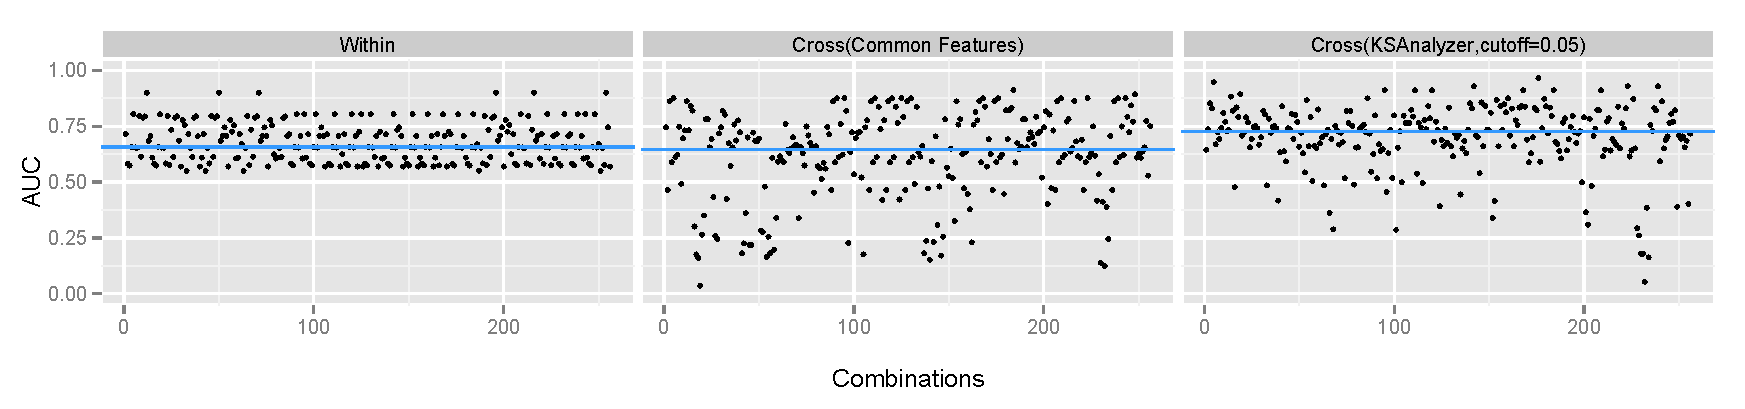
\includegraphics[width=\linewidth]{Figures/Result/auc_compare.pdf}
% 	\caption{Prediction performance comparison among within-results, cross-results
% 	by ASAnalyzer, random analyzer, and manual matching in terms of median AUC values.}
% 	\label{fig:compare_results_on_defect}
% \end{figure*}
% 
% In addition, the median AUC value of all predictions using all defect source
% groups (Defect All in Table~\ref{tab:compare}) is
% 0.701, which is a promising result since the median AUC values in
% within-predictions and cross-predictions by random analyzer and manual matching
% are 0.676, 0.599, and 0.609, respectively. In the case of AEEEM, the median AUC
% of manual feature matching is fairly high (0.673). However, the median AUC of
% within-prediction (0.675) outperforms that of manual feature matching with
% statistical significance (p=0.000).
% 
% Figure~\ref{fig:compare_results_on_defect} shows how each prediction performance
% of within- and cross-predictions varies. The solid line in
% Figure~\ref{fig:compare_results_on_defect} represents the overall prediction
% performance and the mean of all the median AUC values of the targets. Comparing
% the cross-results of AS to within-prediction results, we observed the
% cross-result is better than the within-result. We also compare cross-prediction
% results of AS, random analyzer, and manual matching as well. As we observe, the
% cross-result of AS outperforms that of both random analyzer and manual matching.
% 
% We conducted t-test (p<0.05) for those overall median AUC values between
% within-predictions and cross-predictions of AS. The cross-result of
% AS outperforms the within-result with statistical significance (p=0.002)
% and outperforms those of random analyzer and manual feature matching (p=0.000).
% Thus, we can confirm RQ2; cross-predictions by ASAnalyzer with the cutoff of
% 0.9 outperform to within-predictions in terms of median AUC in our
% experimental setting.


%\begin{result}
%Therefore, we can
%conclude that our cross-domain prediction model can predict defects in targets
%with high coverage
%\end{result}

%--------------------------------------------------------------
% \subsection{Within vs. Cross in non-defect$\Rightarrow$defect}
%--------------------------------------------------------------

% \begin{table}[t]
% \small
% \centering
% \caption{Average AUCs of Within and Cross-prediction results ASAnalyzer with
% Filters and Random Analyzer) by each
% source group in non-defect$\Rightarrow$defect.}
% \label{tab:compare_non_defect}
% \begin{tabular}{|c|c|c|c|c|}
% \hline
% 
% \multirow{2}{*}{\specialcell{{\bf Source}\\{\bf group}}}	&
% \multirow{2}{*}{{\bf Within}}	& \multicolumn{2}{c|}{{\bf Cross}}	&
% \multirow{2}{*}{\specialcell{{\bf Target}\\{\bf coverage}}}
% \\
% 
% \cline{3-4}
% 		& 	& \specialcell{{\bf ASw/F}} & {\bf Random} & \\ \hline
% 
% Effort & 0.63	& 0.84 & 0.73	& 11\% (3/28)\\ \hline
% Severity & N/A  & N/A	& N/A	& 0\% (0/28)\\ \hline
% {\bf SE all}  & {\bf0.63}	& {\bf 0.84} & {\bf 0.73}		& {\bf 11\%} (3/28)\\
% \hline \hline \hline
% Medical	& 0.69	& 0.71	& 0.58	& 32\% (9/28)\\ \hline
% Wine	& 0.57	& 0.55	& 0.57	& 4\% (1/28)\\ \hline \hline
% {\bf non-SE All} & {\bf 0.68}	& {\bf 0.70} & {\bf 0.58}	& {\bf 36\%} (10/28)\\
% \hline
% 
% %{\bf Non-defect All} &{\bf 0.67}	&{\bf 0.73}	&{\bf 0.61} &  \\ \hline
% \end{tabular}
% \end{table}

% Table~\ref{tab:compare_non_defect} shows cross-prediction results in
% non-defect$\Rightarrow$defect in terms of average AUC by each source group.
% Cross-results outperform within-results in non-defect$\Rightarrow$defect as
% well. We conducted the paired t-test for predictions in
% non-defect$\Rightarrow$defect. From the paired t-test, we could conclude that
% cross-results of ASAnalyzer with Filters were comparable to within-results.
% However, we observed very low prediction coverage; 3\% by SE and
% 36\% by non-SE. Thus, we may not generalize this observation, (In
% Section~\ref{sec:prediction_coverage}, we discuss prediction coverage in detail.)
% 
% Random analyzer in Effort in
% Table~\ref{tab:compare_non_defect} outperforms within-predictions in terms of
% average AUC. Note that its within-result is fairly low (0.63). In addition,
% Random analyzer result did not outperform the within-result with statistical significance
% (p=0.18).
% 
% 
% \begin{figure}[t]
% 	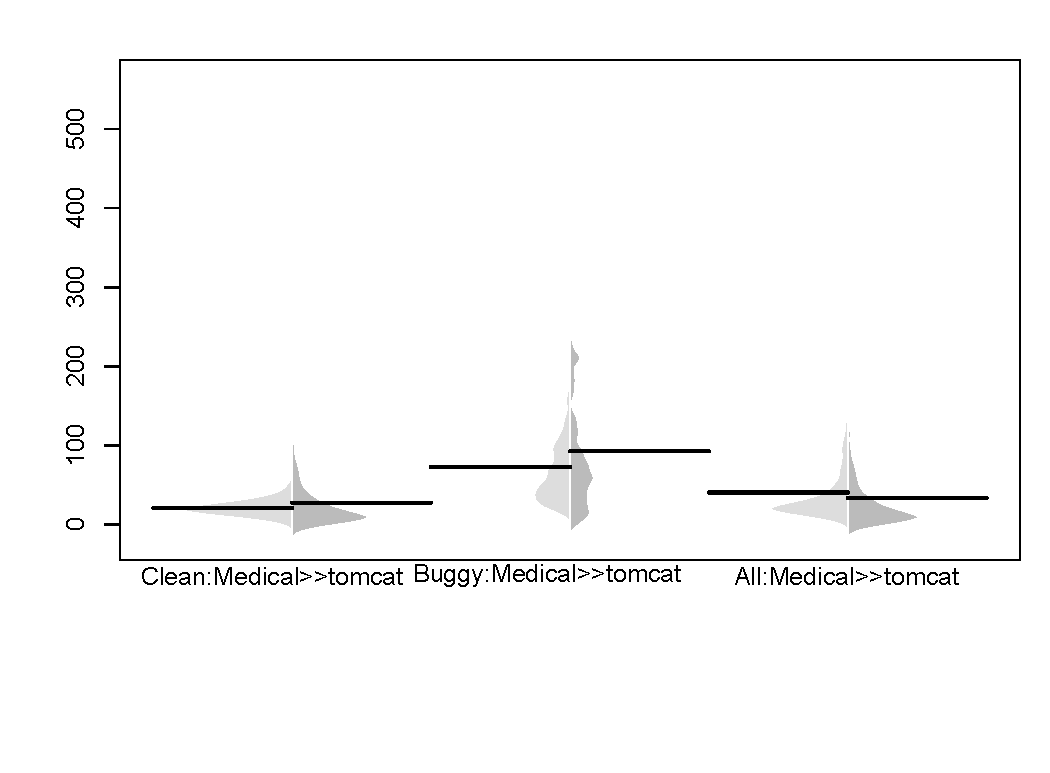
\includegraphics[width=\linewidth]{Figures/Result/medical_dist.pdf}
% 	\caption{Feature distribution of an matched feature from the prediction
% 	combination, Medical(area\_se)$\Rightarrow$Tomcat(rfc), of AUC=0.82.}
% 	\label{fig:medical_dist}
% \end{figure}
% 
% 
% We observed interesting results in Medical. Nine
% out of 28 targets in non-SE$\Rightarrow$defect predictions were covered by
% models from the Medical dataset. An example matched feature is standard error of
% nuclear area of cells (area\_se) of Medical and response for class
% (rfc, to measure coupling) of pc3 in NASA. The area\_se feature represents how
% much irregular the areas of cells are. The higher value of area\_se indicates the higher
% malignancy~\cite{Street93}. This characteristic of the feature, area\_se, is
% similar to that of typical features in defect datasets, as shown in
% Figure~\ref{fig:medical_dist}. We can clearly observe similar distribution
% between the matched features. In addition, original task of the Medical dataset
% was binary classification like software defect prediction in our experimental
% setting. This leads to a bit higher prediction coverage than SE datasets.
% 
% % However, models built by the Wine dataset covered only one target, ar1. This
% % poor coverage of Wine is also due to different characteristics of features from
% % that of typical features used in defect datasets.
% In Wine, ASAnalyzer with Filters is even worse than Random analyzer. In
% addition, models built by the Wine dataset covered only one target.
% Possible explanation is that features in Wine may have different characteristics
% from those in defect datasets and prediction task of Wine is multi-class
% classification rather than binary classification. This may lead
% to different results comparing to that of defect$\Rightarrow$defect.
% 
% For RQ2, we conducted paired t-test for non-defect$\Rightarrow$defect in terms
% of average AUC. Actually, cross-predictions were comparable to
% within-predictions with statistical significant (p=0.15). However, it is hard to
% generalize our result since prediction coverage is very low to conclude RQ2.

% \subsection{Prediction Coverage}
% \label{sec:prediction_coverage}
% 
% % Thus, we could confirm RQ1 in terms of
% % average AUC in our experimental setting. However, we could not confirm RQ3 since
% % prediction coverage of non-defect$\Rightarrow$defect predictions, were too low to compare results.
% 
% 
% \begin{table}[t]
% \small
% \centering
% \caption{Prediction Coverage of ASAnalyzer with Filters (cutoff>0.9) on
% defect$\Rightarrow$defect vs. non-defect$\Rightarrow$defect datasets in terms of
% average AUC.}
% \label{tab:prediction_coverage}
% %\setlength{\tabcolsep}{5pt}
% %\setlength{\extrarowheight}{1.5pt}
% \begin{tabular}{|c|@{ }c@{ }||@{ }c@{ }|@{ }c@{ }|}
% \hline
% \multirow{2}{*}{Target}	& \multirow{2}{*}{defect$\Rightarrow$defect} &
% \multicolumn{2}{c|}{non-defect$\Rightarrow$defect} \\ \cline{3-4}
% & 	& SE$\Rightarrow$defect &
% non-SE$\Rightarrow$defect \\\hline \hline
% EQ			&\cmark	&-&-	\\ \hline
% JDT			&\cmark	&-&\cmark	\\ \hline
% LC			&\cmark	&-&-\\ \hline
% ML			&\cmark	&-&-	\\ \hline
% PDE			&\cmark	&-&-	\\ \hline \hline
% 
% Apache		&\cmark	&-&-	\\ \hline
% Zxing		&\cmark	&-&\cmark	\\ \hline
% Safe		&\cmark	&-&\cmark\\ \hline \hline
% 
% ant-1.3		&\cmark	&-&-	\\ \hline
% arc			&\cmark	&-&-	\\ \hline
% camel-1.0	&\cmark	&-&-	\\ \hline
% poi-1.5		&\cmark	&-&-	\\ \hline
% redaktor	&\cmark	&-&-	\\ \hline
% skarbonka	&\cmark	&-&-	\\ \hline
% tomcat		&\cmark	&- &\cmark	\\ \hline
% velocity-1.4	&\cmark	&-&-	\\ \hline
% xalan-2.4	&\cmark	&-&-	\\ \hline
% xerces-1.2	&\cmark	&-&-	\\ \hline \hline
% 
% cm1			&\cmark	&-&\cmark	\\ \hline
% mw1			&\cmark	&\cmark&\cmark	\\ \hline
% pc1			&\cmark	&-&-	\\ \hline
% pc3			&\cmark	&-&-	\\ \hline
% pc4			&\cmark	&-&\cmark	\\ \hline \hline
% 
% ar1		&\cmark	&-&\cmark	\\ \hline
% ar3		&\cmark	&\cmark&\cmark	\\ \hline
% ar4		&\cmark	&-&\cmark	\\ \hline
% ar5		&\cmark	&\cmark&	\\ \hline
% ar6		&\cmark	&-&-	\\ \hline \hline
% Total & 28/28 (100\%) & 3/28 (11\%) & 10/28 (36\%) \\ \hline

% EQ	&12	&12	\\ \hline
% JDT	&14	&5	\\ \hline
% LC	&12	&11	\\ \hline
% ML	&16	&0	\\ \hline
% PDE	&13	&4	\\ \hline
% 
% Apache	&13	&4	\\ \hline
% Zxing	&20	&18	\\ \hline
% Safe	&17	&12	\\ \hline
% 
% ant-1.3	&9	&9	\\ \hline
% arc	&6	&5	\\ \hline
% camel-1.0	&9	&8	\\ \hline
% poi-1.5	&5	&2	\\ \hline
% redaktor	&10	&0	\\ \hline
% skarbonka	&11	&11	\\ \hline
% tomcat	&6	&4	\\ \hline
% velocity-1.4	&7	&1	\\ \hline
% xalan-2.4	&7	&1	\\ \hline
% xerces-1.2	&9	&0	\\ \hline
% 
% cm1	&17	&16	\\ \hline
% mw1	&9	&9	\\ \hline
% pc1	&14	&4	\\ \hline
% pc3	&12	&1	\\ \hline
% pc4	&15	&0	\\ \hline
% 
% ar1	&15	&15	\\ \hline
% ar3	&17	&16	\\ \hline
% ar4	&16	&16	\\ \hline
% ar5	&14	&12	\\ \hline
% ar6	&11	&10	\\ \hline \hline
% Total & 336 (28) & 206 (24) \\ \hline
% \end{tabular}
% \end{table}

% We checked prediction coverage of our framework for cross-domain defect
% prediction in detail. As shown in Table~\ref{tab:prediction_coverage}, all the
% targets in defect$\Rightarrow$defect could be predicted by our framework. This shows
% prediction coverage of our framework is 100\% in our experimental setting. To
% achieve 100\% coverage, there should exist matched features with high matching
% score ($>$0.9) and the prediction combinations should remain after applying LBM and DM filters. Thus,
% prediction coverage in defect$\Rightarrow$defect clearly shows that features of
% defect datasets could be transferred to build a prediction model and our
% framework could find matched features in defect$\Rightarrow$defect
% predictions.
% 
% However, non-defect$\Rightarrow$defect predictions lead to poor prediction
% coverage. In SE$\Rightarrow$defect prediction, three target projects, mw1, ar3,
% and ar5 are predicted by the framework. This low
% coverage is because of different characteristics of features between defect and
% non-defect datasets. Only three out of all combinations in SE$\Rightarrow$defect
% had co-occurrence features whose matching scores are higher than 0.9. In case
% of the Severity dataset, there were no matched features at all since features of
% the Severity dataset, created by text mining technique such as
% tf*idf~\cite{Menzies08}, are different from typical defect prediction features.


%This poor results in non-defect$\Rightarrow$defect predictions are obvious
% since datasets are collected in too different domains such as severity of
% issue reports and wine quality. We will discuss about this result more,
% particularly, ar5 in SE$\Rightarrow$defect in Section~\ref{sec:Discussion}.
% 
% Somebody may claim the high coverage of defect$\Rightarrow$defect is because of
% many source projects which can make more prediction combinations. In
% non-defect$\Rightarrow$defect predictions, we have few source projects (4)
% comparing to those (15-25) in defect$\Rightarrow$defect predictions for a
% target. However, before applying the HC filter, about 56\% of targets in average
% were already covered by each defect source dataset. This implies that we may
% cover all targets by two or three defect source datasets. In the same setting,
% average prediction coverage by SE and non-SE sources was about 5\% and 18\% respectively.
% 
% In our experimental settings, we could conclude about RQ3:
% \squishlist
% 	\item Our framework for
% cross-domain defect prediction could achieve 100\% prediction coverage in
% defect$\Rightarrow$defect predictions.
% 	\item Non-defect$\Rightarrow$defect predictions are hard to achieve good
% 	prediction coverage since features from different areas are most likely
% 	different from typical features of defect datasets. However, if there exist
% 	datasets whose feature characteristic is similar to that of typical features
% 	from defect datasets and prediction task is similar,i.e. binary classification,
% 	we can increase prediction coverage.
% \squishend
% 
% Due to the low prediction coverage of non-defect$\Rightarrow$defect, we
% only report detailed prediction results of defect$\Rightarrow$defect in
% next sub-sections.


\subsection{Win/Tie/Loss Results}
\label{subsec03}
\begin{table}[!t]
%\small
%\scriptsize
\centering
\caption{Win/Tie/Loss results of HDP by KSAnalyzer (cutoff=0.05)
against WPDP (Baseline1), CPDP-CM (Baseline2), and CPDP-IFS (Baseline3).}
\label{tab:win_results}
%\setlength{\tabcolsep}{5pt}
%\setlength{\extrarowheight}{1.5pt}
%\begin{tabular}{|@{ }c@{ }||@{ }c@{ }|@{ }c@{ }|@{ }c@{ }||@{ }c@{ }|@{ }c@{
%}|@{ }c@{ }|}
\begin{tabular}{|@{}c@{}||@{}c@{}|@{}c@{}|@{}c@{}||@{}c@{}|@{}c@{}|@{}c@{}||@{}c@{}|@{}c@{}|@{}c@{}|}
\hline

\multirow{3}{*}{{\bf Target}}
&\multicolumn{9}{c|}{\bf Against}
\\ \cline{2-10}
&\multicolumn{3}{c||}{\specialcell{{\bf WPDP}\\{(Baseline1)}}}
&\multicolumn{3}{c||}{\specialcell{{\bf CPDP-CM}\\{(Baseline2)}}}
&\multicolumn{3}{c|}{\specialcell{{\bf CPDP-IFS}\\{(Baseline3)}}}
\\
\cline{2-10}

& Win & Tie & Loss & Win & Tie & Loss & Win & Tie & Loss \\ \hline \hline
EQ	&4	&0 	&0	&1	&3 	&0	&4	&0 	&0\\ \hline
JDT	&0	&0 	&5	&3	&0 	&2	&5	&0 	&0\\ \hline
LC	&6	&0 	&1	&3	&3 	&1	&3	&1 	&3\\ \hline
ML	&0	&0 	&6	&4	&2 	&0	&6	&0 	&0\\ \hline
PDE	&4	&0 	&1	&2	&0 	&3	&5	&0 	&0\\ \hline
Apache	&6	&0 	&6	&8	&0 	&4	&10	&0 	&2\\ \hline
Safe	&16	&0 	&3	&14	&0 	&5	&16	&0 	&3\\ \hline
Zxing	&5	&0 	&0	&4	&0 	&1	&4	&1 	&0\\ \hline
ant-1.3	&11	&0 	&0	&7	&0 	&4	&10	&0 	&1\\ \hline
arc	&2	&1 	&0	&2	&0 	&1	&3	&0 	&0\\ \hline
camel-1.0	&5	&0 	&2	&5	&0 	&2	&6	&0 	&1\\ \hline
poi-1.5	&3	&0 	&1	&3	&1 	&0	&3	&0 	&1\\ \hline
redaktor	&0	&0 	&4	&2	&0 	&2	&3	&0 	&1\\ \hline
skarbonka	&15	&0 	&0	&4	&1 	&10	&13	&0 	&2\\ \hline
tomcat	&0	&0 	&1	&1	&0 	&0	&1	&0 	&0\\ \hline
velocity-1.4	&0	&0 	&6	&2	&0 	&4	&2	&0 	&4\\ \hline
xalan-2.4	&0	&0 	&1	&1	&0 	&0	&1	&0 	&0\\ \hline
xerces-1.2	&0	&0 	&2	&2	&0 	&0	&1	&0 	&1\\ \hline
cm1	&8	&0 	&2	&8	&0 	&2	&9	&0 	&1\\ \hline
mw1	&6	&0 	&1	&5	&0 	&2	&5	&0 	&2\\ \hline
pc1	&1	&0 	&6	&6	&0 	&1	&7	&0 	&0\\ \hline
pc3	&0	&0 	&7	&7	&0 	&0	&7	&0 	&0\\ \hline
pc4	&0	&0 	&8	&5	&0 	&3	&8	&0 	&0\\ \hline
jm1	&1	&0 	&5	&5	&0 	&1	&6	&0 	&0\\ \hline
pc2	&5	&0 	&0	&5	&0 	&0	&5	&0 	&0\\ \hline
pc5	&0	&0 	&1	&1	&0 	&0	&1	&0 	&0\\ \hline
mc1	&1	&0 	&0	&1	&0 	&0	&1	&0 	&0\\ \hline
mc2	&16	&0 	&2	&17	&0 	&1	&16	&0 	&2\\ \hline
kc3	&10	&0 	&1	&8	&0 	&3	&10	&0 	&1\\ \hline
ar1	&14	&0 	&0	&14	&0 	&0	&11	&0 	&3\\ \hline
ar3	&17	&0 	&0	&9	&0 	&8	&13	&1 	&3\\ \hline
ar4	&17	&0 	&0	&16	&0 	&1	&16	&0 	&1\\ \hline
ar5	&19	&0 	&3	&17	&2 	&3	&17	&0 	&5\\ \hline
ar6	&8	&1 	&7	&11	&3 	&2	&13	&0 	&3\\ \hline
Total	&\specialcell{{200}\\{70.4\%}}	&\specialcell{{2}\\{0.7\%}}	&\specialcell{{82}\\{28.9\%}}	&\specialcell{{203}\\{71.5\%}}	&\specialcell{{15}\\{5.3\%}}	&\specialcell{{66}\\{23.2\%}}	&\specialcell{{241}\\{84.9\%}}	&\specialcell{{3}\\{1.1\%}}	&\specialcell{{40}\\{14.1\%}}\\ \hline

%Total & \specialcell{{147}\\{66.2\%}} &\specialcell{{3}\\{1.4\%}}
%&\specialcell{{72}\\{32.4\%}}
%& \specialcell{{147}\\{66.2\%}} &\specialcell{{14}\\{6.3\%}}
%&\specialcell{{61}\\{27.5\%}}
%& \specialcell{{182}\\{82.0\%}} &\specialcell{{3}\\{1.3\%}}
%&\specialcell{{37}\\{16.7\%}}
%\\
%\hline
\end{tabular}
\end{table}


To investigate our performance evaluation for HDP in detail, we report
the Win/Tie/Loss results of HDP by KSAnalyzer with the cutoff of 0.05 against
WPDP (Baseline1), CPDP-CM (Baseline2), and CPDP-IFS
(Baseline3) in Table~\ref{tab:win_results}.


KSAnalyzer with the cutoff of 0.05 conducted 284 out of 962 prediction
combinations since 584 combinations do not have any matched
metrics because of the cutoff threshold. In
Table~\ref{tab:win_results}, the target dataset, EQ, was predicted in four
prediction combinations and our approach, HDP, outperforms Baseline1 and
Baseline3 in the four combinations (i.e. 4 Wins). However, HDP outperforms
Baseline2 in only one combinations of the target, EQ (1 Wins). 


% \subsection{Matched features}
% In this section, we discuss matched features to investigate prediction
% performance on cross-domain defect prediction in detail.

% A reason why ASAnalyzer can predict defects pretty well on cross-domain
% settings is that most defect prediction metrics usually represent complexity of
% source code and its change; it tends to be more buggy when the complexity is
% higher.
Against Baseline1, the six targets such as EQ, Zxing, ant-1.3, skarbonka, pc2, 
mc1, ar1, ar3, and ar4 have only Win results. In other words, defects in those nine targets
could be predicted better by other source projects using HDP models by
KSAnalyzer compared to WPDP models.

\label{sec:why}
\begin{figure}[t]
	\centering
	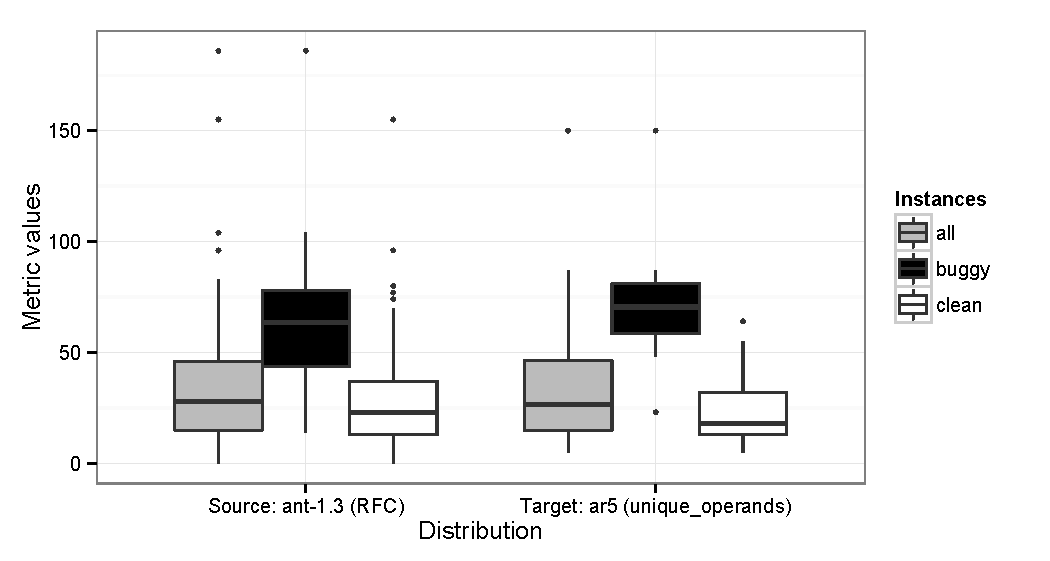
\includegraphics[width=\linewidth]{Figures/Result/best_dist_bplot.pdf}
	\caption{Distribution of metrics (matching score=0.91)
	from ant-1.3$\Rightarrow$ar5 (AUC=0.946).}
	\label{fig:best_dist}
\end{figure}

In Figure~\ref{fig:best_dist}, we analyzed distributions of matched metrics using box plots for one of Win cases, ant-1.3$\Rightarrow$ar5. 
% the feature value distribution of
% a matched feature in the prediction combination, ant-1.3$\Rightarrow$ar5, whose AUC is 0.938.
The gray, black, and white box plots show distributions of matched metric values in
all, buggy, and clean instances respectively. The three box plots on the
left-hand side represent distributions of a source metric while the three
box plots on the right-hand side represent those of a target metric. The
bottom and top of the boxes represent the first and third quartiles
respectively.
The solid horizontal line in a box represents the median metric value in each distribution. 
Black points in the figure are outliers.

Figure~\ref{fig:best_dist} explains how the prediction
combination of ant-1.3$\Rightarrow$ar5 can have a high AUC, 0.946. Suppose
that a simple model predicts that an instance is buggy when the metric value of
the instance is more than 40 in the case of Figure~\ref{fig:best_dist}. In both
datasets, approximately 75\% or more buggy and clean instances will be
predicted correctly. In Figure~\ref{fig:best_dist}, the matched metrics in
ant-1.3$\Rightarrow$ar5 are the response for class ({\em RFC}: number of methods
invoked by a class)~\cite{Chidamber94} and the number of unique operands ({\em
unique\_operands})~\cite{Halstead77}, respectively. The {\em RFC} and {\em
unique\_operands} are not the same metric so it might look like an arbitrary
matching. However, they are matched based on their similar distributions as
shown in Figure~\ref{fig:best_dist}. Typical defect prediction metrics have
tendencies in which higher complexity causes more
bug-proneness~\cite{DAmbros12,Menzies07,Rahman13}. In
Figure~\ref{fig:best_dist}, instances with higher values of {\em RFC} and {\em
unique\_operands} have the tendency to be more bug-prone. For this reason, the
model using the matched metrics could achieve such a high AUC (0.946). We could
observe this bug-proneness tendency in other Win results. Since matching metrics is
based on similarity of source and target metric distributions, HDP also
addresses several issues related to a dataset shift such as the covariate shift
and domain shift discussed by Turhan~\cite{Turhan12}.

%The Win/Tie/Loss results show that with our HDP model by KSAnalyzer there is a higher possibility of getting a better prediction performance.


%%%%%%%%
% LOSS results
%%%%%%%
However, there are still about 28.9\% Loss results against WPDP as shown in Table~\ref{tab:win_results}. The eight targets such as JDT, ML, redaktor, tomcat, velocity-1.4, xalan-2.4,
xerces-1.2, pc3, pc4, and pc5 have no Wins at all against Baseline1. In
addition, other targets still have Losses even though they have Win or Tie
results.


\begin{figure}[t]
	\centering
	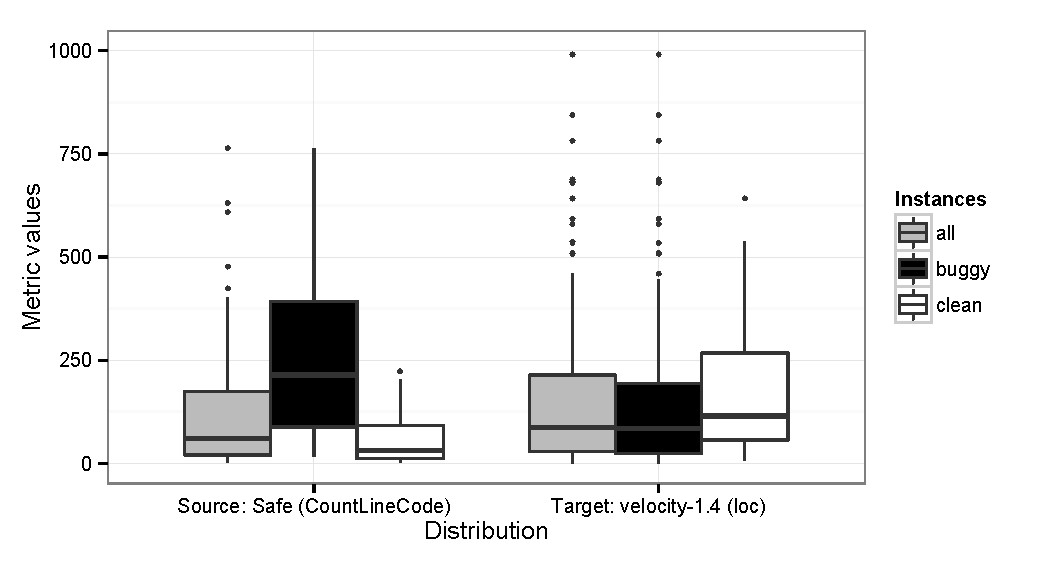
\includegraphics[width=\linewidth]{Figures/Result/loss_dist_bplot.pdf}
	\caption{Distribution of metrics (matching score=0.45)
	from Safe$\Rightarrow$velocity-1.4 (AUC=0.391).}
	\label{fig:loss_dist}
\end{figure}


As a representative Loss case, we investigated distributions of the matched metrics in Safe$\Rightarrow$velocity-1.4, whose AUC is 0.391.
As observed, Loss results were usually caused by different tendencies of
bug-proneness between source and target metrics. Figure~\ref{fig:loss_dist}
shows how the bug-prone tendencies of source and target metrics are different.
Interestingly, the matched source and target metric by the KSAnalyzer is the
same as {\em LOC} ({\em CountLineCode} and {\em loc}) in both.
As we observe in the figure, the median metric value of buggy instances is higher than that of clean instances in that the more {\em LOC}
implies the higher bug-proneness in the case of Safe. However, the median metric value of
buggy instances in the target is lower than that of clean instances
in that the less {\em LOC} implies the higher bug-proneness in
velocity-1.4. This inconsistent tendency of
bug-proneness between the source and target metrics could degrade the
prediction performance although they are the same metric.

We regard the matching that has an inconsistent bug-proneness tendency between
source and target metrics as a noisy metric matching.
% This implies the target
% feature does not follow the tendency that a higher complexity causes more bug-proneness.
% The target feature worked as noise when the model predicted
% defects in velocity-1.4. 
We could observe this kind of noisy metric matching in
prediction combinations in other Loss results.

However, it is very challenging to filter out the noisy metric matching since we
cannot know labels of target instances in
advance. If we could design a filter for the noisy metric matching, the Loss
results would be minimized. Thus, designing a new filter to mitigate these Loss
results is an interesting problem to address. Investigating this new filter
for the noisy metric matching will remain as future work.

Figure~\ref{fig:loss_dist} also explains why CPDP-CM did not show reasonable
prediction performance. Although the matched metrics are same
as {\em LOC}, its bug-prone tendency is inconsistent. Thus, this matching using
the common metric was noisy and was not helpful for building a prediction model.

% The DM filter could not remove
% this matched feature since the modality of all instances in both source and
% target is still similar. Without knowing labels of target instances, it is
% difficult to filter out this case. Other Loss results also have similar
% observations. Designing new filters for these Loss results is a challenging
% issue since we cannot know distribution of clean and buggy instances of target in
% advance. Investigating new filters for these patterns remains as future work.



% The pc4 in Table~\ref{tab:win_results} also have many Loss results.
% However, note that pc4 still have very high AUC values, 0.899 and 0.70,
% respectively, The AUC value of 0.70 is considered as a promising result in defect prediction~\cite{Giger12, Lessmann08}. The reason for Loss results
% of pc1 and pc3 is that within-results in AUC are already very high, 0.78 and
% 0.79, respectively.


%\TODO{Guidelines or suggestions on cross-domain defect prediction?}

Overall, the numbers of Win and
Tie results are 200 and 2 respectively out of all of the 284 prediction
combinations.
This means that in 71.1\% of prediction combinations our HDP
models achieve better or comparable prediction performance than those in
WPDP.

The Win/Tie/Loss results against Baseline2 and Baseline3 show a similar trend.
In the 218 (76.8\%) out of 284 prediction combinations, HDP outperforms and is comparable to CPDP-CM. Against Baseline3, 244
(85.9\%) prediction combinations are Win or Tie results.

%A recent study shows that high defect rate of a dataset may bias prediction results,i.e., higher buggy rate of a dataset tends to lead better prediciton results~\cite{Tantithamthavorn16}. This bias could be matter under the WPDP setting as the study discusses about model validation technioques~\cite{Tantithamthavorn16}. Since HDP is CPDP on datasets using different metric sets, To make sure if the promising reuslts of HDP is affected by the defect rate of a target dataset


\subsection{Performance in Different Metric Selections}
\label{subsec04}

\begin{table}[!t]
%\small
%\scriptsize
\centering
\caption{Prediction performance (a
median AUC and \% of Win) in different metric selections.
% Between within- and
% cross-results by
% analyzers, outperforming results with statistical significance
% (Wilcoxon signed-rank, p$<$0.05) is bold-faced. Between cross-results using
% common features and by analyzers, outperforming results with
% statistical significance (Wilcoxon signed-rank, p$<$0.05) is underlined.}
}
\label{tab:various_fs}
%\setlength{\tabcolsep}{5pt}
%\setlength{\extrarowheight}{1.5pt}
\begin{tabular}{|@{}c@{}||c@{ }|c@{}||c@{ }|c@{}||c@{ }|c@{}||c|}
%\begin{tabular}{|@{ }c@{ }||c|c||c|c||c|c||c|}
\hline
\multirow{3}{*}{\bf{Approach}}
&\multicolumn{6}{@{ }c@{ }||}{\bf Against}
&\multirow{2}{*}{\specialcell{\bf{HDP}}}
\\\cline{2-7}
&\multicolumn{2}{@{ }c@{ }||}{\specialcell{\bf{WPDP}}}
&\multicolumn{2}{@{ }c@{
}||}{\specialcell{\bf{CPDP-CM}}}
&\multicolumn{2}{@{ }c@{ }||}{\specialcell{\bf{CPDP-IFS}}}
&
\\
\cline{2-8}
& \bf{AUC}
& \bf{Win\%}
& \bf{AUC}  
& \bf{Win\%}
& \bf{AUC}  
& \bf{Win\%}
& \bf{AUC}  
\\
\hline
\hline
Gain Ratio	& 0.654 &70.4\%	&0.632 &71.5\% &0.558 &84.9\% &0.718	\\ \hline
Chi-Square	& 0.645 &70.2\%	&0.635 &70.8\% &0.557 &86.2\% &0.720  \\ \hline
Significance& 0.654 &70.7\%	&0.630 &71.4\% &0.557 &86.6\% &0.718  \\ \hline
Relief-F		& 0.663 &63.1\%	&0.642 &68.1\% &0.540 &83.3\% &0.709	\\ \hline
None			& 0.657 &61.3\%	&0.622 &65.5\% &0.545 &78.8\% &0.701	\\ \hline
\end{tabular}
\end{table}

Table~\ref{tab:various_fs} shows prediction results on various metric selection approaches
including with no metric selection (`None'). We compare the median AUCs of
the HDP results by KSAnalyzer with the cutoff of 0.05 to those of WPDP, CPDP-CM,
or CPDP-IFS, and report the percentages of Win results.

Overall, we could observe metric selection to be helpful in improving
prediction models in terms of AUC. When applying metric selection, the Win results
account for more than about 63\% in most cases against WPDP and CPDP-CM. Against
CPDP-IFS, the Win results of HDP account for more than 83\% after applying the
metric selection approaches. This implies that the metric selection approaches
can remove irrelevant metrics to build a better prediction model. In addition, this result confirms
the previous studies that we can build prediction models better than or
comparable to WPDP models with even a few key metrics~\cite{Gao11, He14subset}.
However, the percentages of Win results in `None' were lower than those in
applying metric selection. Among metric selection approaches, `Gain Ratio', `Chi-Square' and
`Significance' based approaches lead to the best performance in terms of the
percentages of the Win results (70.2\%-70.7\%) against WPDP.

\subsection{Performance in Various Metric Matching Analyzers}
\label{subsec05}
% \begin{table*}[t]
% \scriptsize
% \centering
% \caption{Prediction performance in other analyzers with the matching
% score cutoff thresholds, 0.05 and 0.90. Significance attribute selection is used
% for metric selection.
% % Between within- and
% % cross-results by
% % analyzers, outperforming results with statistical significance
% % (Wilcoxon signed-rank, p$<$0.05) is bold-faced. Between cross-results using
% % common features and by analyzers, outperforming results with
% % statistical significance (Wilcoxon signed-rank, p$<$0.05) is underlined.}
% }
% \label{tab:other_analyzers}
% %\setlength{\tabcolsep}{5pt}
% %\setlength{\extrarowheight}{1.5pt}
% %\begin{tabular}{|@{ }c@{ }|@{ }c@{ }||@{ }c@{ }||@{ }c@{ }|@{ }c@{ }|@{ }c@{
% %}||@{ }c@{ }||@{ }c@{ }|@{ }c@{ }|@{ }c@{ }||@{ }c@{ }||@{ }c@{ }|}
% \begin{tabular}{|c|c||c|c|c|c||c|c|c|c||c||c|}
% \hline
% \multirow{2}{*}{\specialcell{\bf{Analyzer}}}
% &\multirow{2}{*}{\specialcell{\bf{Threshold}}}
% &\multicolumn{4}{c||}{\textbf{Against WPDP}}
% &\multicolumn{4}{c||}{\specialcell{\bf{Against CPDP}\\\bf{using Common Metrics}}}
% &\specialcell{\bf{HDP by\\analyzers}}
% &\multirow{2}{*}{\specialcell{\bf{Target}\\\bf{Coverage}}}
% \\\cline{3-11}
% &
% & \bf{AUC}
% & \bf{Win\%}
% & \bf{Tie\%}
% & \bf{Loss\%}
% & \bf{AUC} 
% & \bf{Win\%}
% & \bf{Tie\%}
% & \bf{Loss\%}
% & \bf{AUC}
% & 
% \\
% \hline
% \hline
% %PAnalyzer& 0.00 & \bf{0.684}	& \underline{0.640}	& 0.606 & 100\% \\ \hline 
% PAnalyzer& 0.05 & \bf{0.684} & 30.3\% & 3.0\% & 66.7\%
% &\underline{0.640} & 45.1\% & 2.2\% & 52.7\%
% & 0.617 & 100\%
% \\
% \hline PAnalyzer& 0.90  & 0.657 & 54.2\% & 2.4\% & 43.4\%
% &0.622 & 65.1\% & 1.2\% & 33.7\%
% & \underline{0.692} & 96\% \\
% \hline
% \hline
% \hline
% 
% %KSAnalyzer & 0.00 & 0.670 &	0.637	& \underline{0.669} & 100\% \\ \hline 
% KSAnalyzer & 0.05 & 0.657 & 66.2\% & 1.4\% & 32.4\% 
% &0.636 & 66.2\% & 6.3\% & 27.5\% 
% &\underline{\bf{0.724}} &100\% \\
% \hline KSAnalyzer& 0.90  & 0.657 & 100\% & 0.0\% & 0.0\%
% &0.761 & 71.4\% & 0.0\% & 28.6\%
% &\bf{0.852}&21\% \\ \hline
% \hline
% \hline
% 
% %SCoAnalyzer & 0.00 & \bf{0.684}	&\underline{0.640}	&0.517 & 100\% \\ \hline 
% SCoAnalyzer & 0.05 & \bf{0.684} & 28.5\% & 1.7\% & 69.8\%
% &\underline{0.640} & 37.3\% & 3.5\% & 59.2\%
% &0.542 & 100\%
% \\
% \hline SCoAnalyzer& 0.90 & \bf{0.684} & 29.0\% & 1.8\% & 69.2\%
% &\underline{0.639} & 36.6\% & 3.3\% & 60.1\%
% &0.547 &
% 100\%
% \\
% \hline
% 
% %PiAnalyzer& 0.00 & \bf{0.684}	&\underline{0.640}	&0.589 & 100\% \\ \hline 
% % PiAnalyzer& 0.05 & \bf{0.684}	&0.582 &25.2\% & 100\% \\ \hline 
% % PiAnalyzer& 0.90 & \bf{0.684}	&0.592 &27.0\% & 100\% \\ \hline
% \end{tabular}
% \end{table*}


\begin{table}[!t]
%\footnotesize
%\scriptsize
\centering
\caption{Prediction performance in other analyzers with the matching
score cutoffs, 0.05 and 0.90. (TgtCov=Target coverage)
% Between within- and
% cross-results by
% analyzers, outperforming results with statistical significance
% (Wilcoxon signed-rank, p$<$0.05) is bold-faced. Between cross-results using
% common features and by analyzers, outperforming results with
% statistical significance (Wilcoxon signed-rank, p$<$0.05) is underlined.}
}
\label{tab:other_analyzers}
%\setlength{\tabcolsep}{5pt}
%\setlength{\extrarowheight}{1.5pt}
%\begin{tabular}{|@{ }c@{ }|@{ }c@{ }||@{ }c@{ }||@{ }c@{ }|@{ }c@{ }|@{ }c@{
%}||@{ }c@{ }||@{ }c@{ }|@{ }c@{ }|@{ }c@{ }||@{ }c@{ }||@{ }c@{ }|}
\begin{tabular}{|@{}c@{}|@{}c@{}||@{}c@{}|@{}c@{}||@{}c@{}|@{}c@{}||@{}c@{}|@{}c@{}||@{}c@{}||@{}c@{}|}
%\begin{tabular}{|c|c||F|F||F|F||F|F||F||c|}
\hline
\multirow{3}{*}{\specialcell{\bf{Analyzer}}}
&\multirow{3}{*}{\bf Cutoff}
&\multicolumn{6}{c||}{\bf Against}
&\multirow{2}{*}{\bf HDP}
&\multirow{3}{*}{\specialcell{\bf{Tgt}\\{\bf Cov}}}
\\ \cline{3-8}

&
&\multicolumn{2}{c||}{\specialcell{\bf{WPDP}}}
&\multicolumn{2}{c@{ }||}{\bf CPDP-CM}
&\multicolumn{2}{c@{ }||}{\bf CPDP-IFS}
&
&
\\\cline{3-9}
&
& \bf{AUC}
& \bf{Win\%}
& \bf{AUC} 
& \bf{Win\%}
& \bf{AUC} 
& \bf{Win\%}
& \bf{AUC}
& 
\\
\hline
\hline
%PAnalyzer& 0.00 & \bf{0.684}	& \underline{0.640}	& 0.606 & 100\% \\ \hline 
P& 0.05 & \bf{-} & -\%
&\underline{-} & -\% 
& -	&-\%
& - & -\%
\\
\hline P& 0.90  & 0.657 & 55.0\% 
&0.629 & 63.6\% 
& 0.558	& 79.3\%
& \underline{0.693}* & 100\% \\
\hline
\hline
\hline

%KSAnalyzer & 0.00 & 0.670 &	0.637	& \underline{0.669} & 100\% \\ \hline 
KS & 0.05 & 0.654 & 70.4\% 
&0.613 & 71.5\% 
& 0.524	&84.9\%
&\underline{\bf{0.724}}* &100\% \\
\hline KS& 0.90  & 0.657 & 77.8\% 
&0.588 & 77.8\% 
& 0.585	&100.0\%
&\underline{0.831}*&21\% \\ \hline
\hline
\hline

%SCoAnalyzer & 0.00 & \bf{0.684}	&\underline{0.640}	&0.517 & 100\% \\ \hline 
SCo & 0.05 & \bf{0.705} & 41.9\%
&0.655 &55.8\%
& 0.520	&68.4\%
&\underline{0.678}* & 100\%
\\
\hline SCo& 0.90 & {\bf 0.705} & 43.4\% 
&0.654 & 53.1\%
&0.520	&69.8\%
&\underline{0.679}*&
100\%
\\
\hline

%PiAnalyzer& 0.00 & \bf{0.684}	&\underline{0.640}	&0.589 & 100\% \\ \hline 
% PiAnalyzer& 0.05 & \bf{0.684}	&0.582 &25.2\% & 100\% \\ \hline 
% PiAnalyzer& 0.90 & \bf{0.684}	&0.592 &27.0\% & 100\% \\ \hline
\end{tabular}
\end{table}



% \begin{table}[t]
% \scriptsize
% \centering
% \caption{Prediction performance in other analyzers with the matching
% score cutoff thresholds, 0.05 and 0.90.
% % Between within- and
% % cross-results by
% % analyzers, outperforming results with statistical significance
% % (Wilcoxon signed-rank, p$<$0.05) is bold-faced. Between cross-results using
% % common features and by analyzers, outperforming results with
% % statistical significance (Wilcoxon signed-rank, p$<$0.05) is underlined.}
% }
% \label{tab:other_analyzers}
% %\setlength{\tabcolsep}{5pt}
% %\setlength{\extrarowheight}{1.5pt}
% \begin{tabular}{|@{ }c@{ }|@{ }c@{ }||@{ }c@{ }|@{ }c@{ }|@{ }c@{ }||@{ }c@{
% }|@{ }c@{ }|@{ }c@{ }|}
% \hline
% {\bf Analyzer} & \bf{threshold} & \bf{Within} & \bf{\specialcell{Cross\\ using\\
% Common \\ Features}} & \bf{\specialcell{Cross by\\ analyzer}} & \bf{coverage}
% \\
% \hline
% \hline
% %PAnalyzer& 0.00 & \bf{0.684}	& \underline{0.640}	& 0.606 & 100\% \\ \hline 
% PAnalyzer& 0.05 & \bf{0.684}	& \underline{0.640}	& 0.617 & 100\% \\ \hline 
% PAnalyzer& 0.90 & 0.657	& 0.622	& \underline{0.692} & 96\% \\ \hline \hline
% \hline
% 
% %KSAnalyzer & 0.00 & 0.670 &	0.637	& \underline{0.669} & 100\% \\ \hline 
% KSAnalyzer & 0.05 & 0.657 &	0.636	& \bf{\underline{0.724}} & 100\% \\ \hline 
% KSAnalyzer& 0.90 & 0.657 &	0.761 &\bf{0.852} & 21\% \\ \hline \hline \hline
% 
% %SCoAnalyzer & 0.00 & \bf{0.684}	&\underline{0.640}	&0.517 & 100\% \\ \hline 
% SCoAnalyzer & 0.05 & \bf{0.684}	&\underline{0.640}	&0.542 & 100\% \\ \hline 
% SCoAnalyzer& 0.90 & \bf{0.684}	&\underline{0.639}	&0.547 & 100\% \\ \hline
% \hline
% \hline
% 
% %PiAnalyzer& 0.00 & \bf{0.684}	&\underline{0.640}	&0.589 & 100\% \\ \hline 
% PiAnalyzer& 0.05 & \bf{0.684}	&\underline{0.640}	&0.582 & 100\% \\ \hline 
% PiAnalyzer& 0.90 & \bf{0.684}	&\underline{0.637}	&0.592 & 100\% \\ \hline
% \end{tabular}
% \end{table}

In Table~\ref{tab:other_analyzers}, we compare the prediction performance in
other analyzers with the matching score cutoff thresholds, 0.05 and 0.90.
HDP's prediction results by PAnalyzer, with a cutoff of 0.90, are
comparable to WPDP. This
implies that comparing 9 percentiles between source and target metrics can
evaluate the similarity of them well with a threshold of 0.90. However,
PAnalyzer with the cutoff is
too simple an approach to lead to better prediction performance than KSAnalyzer. In
KSAnalyzer with a cutoff of 0.05, the AUC (0.724) outperforms it (0.693) in WPDP
with statistical significance.

HDP by KSAnalyzer with a cutoff of 0.90 could lead to significant
improvement in the AUC value (0.831) compared to that (0.724) with the
cutoff of 0.05.
However, the target coverage is just 21\%. This is because some prediction
combinations are automatically filtered out since poorly matched metrics, whose
matching score is not greater than the cutoff, are ignored. In other words,
defect prediction for 79\% of targets was not
conducted since the matching scores of matched metrics in prediction
combinations for the targets are not greater than 0.90 so
that all matched metrics in the combinations were ignored.

An interesting observation in PAnalyzer and KSAnalyzer is that AUC
values of HDP by those analyzers improved when a cutoff threshold
increased. As the cutoff threshold increased as 0.05, 0.10, 0.20,\ldots, and
0.90, we observed prediction results by PAnalyzer and KSAnalyzer
gradually improved from \jc{0.617} to 0.693 and 0.724 to 0.831 in AUC, respectively.
This means these two analyzers can filter out negative prediction combinations
well. As a result, the percentages of Win results are also significantly
increased.

Results by SCoAnalyzer were
worse than WPDP results. In addition,
prediction performance rarely changed regardless of cutoff thresholds; results
by SCoAnalyzer in different cutoffs from 0.05 to 0.90 did not
vary as well.
A possible reason is that SCoAnalyzer does not directly compare
the distributions between source and target metrics.
This result implies that the similarity of distribution between source and
target metrics is a very important factor for building a better
prediction model.


\subsection{Performance in Various Machine Learners}
\label{subsec06}
\begin{table}[!t]
%\small
%\scriptsize
\centering
\caption{Win/Tie percentages of HDP by KSAnalyzer (cutoff=0.05)
against WPDP, CPDP-CM, and CPDP-IFS by different machine learners.}
\label{tab:diff_learners}
%\setlength{\tabcolsep}{5pt}
%\setlength{\extrarowheight}{1.5pt}
%\begin{tabular}{|c||m{1.5cm}|m{1.5cm}|m{1.5cm}||m{1.5cm}|m{1.5cm}|m{1.5cm}|}
\begin{tabular}{|c@{ }||c@{ }|c@{ }||c@{ }|c@{ }||c@{ }|c@{ }|}
\hline
\multirow{3}{*}{\specialcell{{\bf HDP}\\{\bf Learners}}}
&\multicolumn{6}{@{ }c@{ }|}{\bf Against}
\\ \cline{2-7}

&\multicolumn{2}{@{ }c@{ }||}{\specialcell{{\bf WPDP}}}
&\multicolumn{2}{@{ }c@{ }||}{\specialcell{{\bf CPDP-CM}}}
&\multicolumn{2}{@{ }c@{ }|}{\specialcell{{\bf CPDP-IFS}}}
\\
\cline{2-7}

& Win & Tie 
& Win & Tie 
& Win & Tie \\ \hline \hline
SimpleLogistic	&70.4\% &0.7\%	&71.5\% &5.3\% 
& 84.9\% &1.1\%   \\ \hline
RandomForest		&38.7\%	&5.3\%	&45.4\% &4.9\% 
& 69.0\% &1.4\% 	\\ \hline
BayesNet			&39.4\%	&6.0\%	&46.5\% &1.1\% 
& 63.0\% &2.8\% 	\\ \hline
%NaiveBayes		&26.1\%	&1.8\%	&71.1\% &54.5\% &3.2\% &42.3\%	\\ \hline
SVM				&6.7\%	&2.1\%	&29.2\% &1.1\% 
& 32.0\% &14.1\% 	\\ \hline
J48				&21.1\% &3.9\%	&36.6\% &2.1\% 
& 43.3\% &8.5\%   \\ \hline
Logistic			&65.5\%	&1.8\% & 68.3\% &4.9\%  
& 82.0\% &2.7\%  	\\ \hline
LMT				&64.1\% &0.7\%	&64.1\% &4.6\% 
& 78.2\% &1.2\%   \\ \hline

\end{tabular}
\end{table}

To investigate if
HDP works with other machine learners, we built HDP models (KSAnalyzer and
the cutoff of 0.05) with various learners used in defect prediction
literature such as Random Forest, BayesNet, SVM, J48 Decision
Tree, Logistic Regression (Logistic),
and Logistic Model Trees
(LMT)~\cite{DAmbros12,Ghotra15,Lee11,Lessmann08,Nam13,Song11,Ghotra15}.
Table~\ref{tab:diff_learners} shows Win/Tie results.

Simple Logistic led to the best results among various
learners. The Simple Logistic builds a linear logistic regression model based on LogitBoost~\cite{Landwehr2005}. It works well when there is a linear
relationship between a predictor variable (a metric) and the logit
transformation of the outcome variable (bug-proneness)~\cite{Landwehr2005,Logstic}.
In our study, this linear relationship is related to the bug-proneness tendency of
a metric, that is, a higher complexity causes more bug-proneness~\cite{DAmbros12,Menzies07,Rahman13}.
As the consistent bug-prone tendency of matched metrics is important in HDP, the
HDP models built by Simple Logistic can lead to the best prediction
performance.

HDP models built by other learners such as
Logistic and LMT led to comparable results to Simple Logistic against
CPDP-CM and CPDP-IFS. Against Baseline2, Win + Tie results in
Logistic and LMT are greater than about 70\%.
%Against Baseline3, the HPD results with Simple
%Logistic and LMT are similar to those with Logistic regression. 
Logistic also uses the logit function and LMT adopts Logistic
Regression at the leaves of decision tree~\cite{Ghotra15}. In other words, both
learners consider the linear relationship like Simple Logistic~\cite{Landwehr2005,Logstic}. In our experimental settings, HDP tends to
work well with the learners based on the linear relationship between a metric
and a label (bug-proneness).

\subsection{Summary}
In Section~\ref{sec:Result}, we showed HDP results for RQ1. The followings are the key observations of the results in our experimental setting:
\squishlist
    \item Overall, HDP led to better or comparable results to the baselines such as WPDP, CPDP-CM, and CPDP-IFS when using KSAnalyzer with the cutoff of 0.05 and significance attribute selection.
    \item Compared to WPDP, HDP achieved 71.1\% of Win/Tie results. However, there are still 28.9\% of Loss results against WPDP. Based on the analysis of distributions of matched metrics, we observed that the Loss cases are caused by the inconsistent defect-proneness tendency of the matched metrics. Identifying the inconsistent tendency in advance is a challenging problem to be solved. 
    \item Applying metric selection approaches could improve HDP performances against the baselines.
    \item KSAnalyzer showed the best HDP performance compared to PAnalyzer and SCoAnalyzer. This confirms that KS-test is a good tool to compare distributions of two variables~\cite{Lilliefors67,Massey51}.
    \item HDP worked well with Simple Logistic, Logistic, and LMT but not other machine learners. One possible reason is that Logistic related classifiers capture the linear relationship between metrics and the logit transformation of labels that is related to the bug-proneness tendency of the metrics.
\squishend
